\documentclass[11pt]{article}

\title{Teknologipr  osjekt: Øving 2}
\author{Mathias Mellemstuen, Tobias Hallingstad, Ruben Fosby, Henrik Bratseth, Andreas Thauland, Erik Holmen}
\date{16.10.20}

\usepackage{graphicx}
\graphicspath{ {./images/} }

\begin{document}
\begin{center}
\section*{Teknologiprosjekt: Øving 2}
\textbf{Planning report}
\line(1,0){400}
\end{center}
The project fits for industrial warehouses, hospitals and anywhere robots are suited to move things around automatically. There is a lack of cheap options in the current state of the art.
\\Our expected outcome is to make a robot follow a painted line, using a camera and detect objects in its path using an ultrasonic range finder. The robot should be able to move on any track and make decisions in real time.
The overall goal is to create a cost-efficient line-following robot that can do simple tasks such as carrying cargo from A to B. The robot should be able work in different scenarios (harbor, warehouse, hospitals etc).
\\\\
\textbf{Requirements}\\
\begin{itemize}
    \item Following any track with specific requirements.
    \item Regulate angular and linear velocity.
    \item Detect obstacles and respond to them. 
    \item Carry small items as cargo.
    \item Control and get values / status in a web interface.
\end{itemize}
\textbf{Limitations}
\\
\begin{itemize}
	\item The robot will stop if it detects an obstacle instead of trying to move past it. 
	\item Can’t carry too heavy/big objects.
	\item The lines in the track must be in a constant color, it must be a contrast between the background and the track. 
\end{itemize}
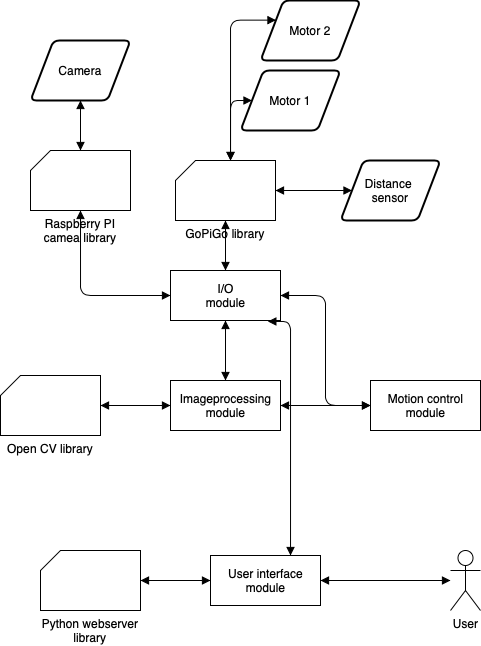
\includegraphics[width=10cm]{flowdiagram}
\\
\textbf{Motion control algorithm}
\\
\begin{enumerate}
    \item Sample input data from the distance sensor and stop the robot if the distance is within a certain value. 
    \item Check data from the image processing if the track exists in the image. \begin{itemize}
        \item On track: Goto point 3. 
        \item Not on track: Drive around in circles until the track is found.
    \end{itemize}
    \item Check if the robot is near a crossroad. \begin{itemize}
        \item On crossroad: Move either left. right or forward. The robot can be hardcoded to always move in one direction or take a random direction. 
        \item Not on crossroad: Go to point 4. 
    \end{itemize}
    \item Find the shortest distance and angle to the middle of the track. This will be the general direction / the next destination. 
    \item Calculate angular and linear velocity according to the data sampled in point 3. 
    \item Check if it has reached it's final destination or goal. If that is not the case, go to point 1.
\end{enumerate}
\textbf{I/O module}
\\
This module contains code for every sensor on the robot, including output to the motors. This module will be responsible for connecting every other module together, it will be the core code of the robot. 
\\\\
\textbf{Camera module}
\\
The project includes a Raspberry Pi camera. We will use the standard raspberry Pi camera library to receive images from the camera. Then we will use OpenCV to convert the image to an array of pixels.
\\\\
\textbf{Distance sensor}
\\ 
The project includes a distance sensor. The GoPiGo library contains a function that returns the distance to the obstacles in millimetres which we can use further in the code. 
\\\\
\textbf{Motor I/O}
\\
A function to control the wheels of the robot. The function should take two parameters, one for the speed of the wheel and another that defines which wheel to set the speed. 
\\\\
\textbf{Image processing module}
\\
\begin{itemize}
    \item Get the image as an array of pixels from the I/O module. 
    \item Convert the colors in the array to black/white.
    \item Use the Hough transform algorithm to find the edges of the track.
    \item Find the middle of the road.
    \item Return the middle of the road and the robots offset to the middle. 
\end{itemize}
\textbf{User interface} 
\\
The user interface is a web page that is locally hosted on the raspberry pi. The webserver is running within the python program. The web page is using API calls to collect data / give command to the python program. All of this is happening asynchronous with the rest of the python code. 
\\\\
\textbf{Installation and deployment of the solution (Implementation)}
\begin{enumerate}
    \item Installing the raspbian OS on a microSD card. 
    \item Setting up the raspberry pi to host a WIFI network. 
    \item Creating users for each group member on the linux system.
    \item Setting up SSH. 
    \item Installing the GoPiGo libraries from github. 
    \item Opening port 80 on the firewall for the web interface. 
    \item Setting up a service in systemctl to run the python code when linux is booting.
\end{enumerate}

Work Package (WP)
Estimated time to finish WP
Responsibility
Planning
x days
x person
Create the Motion control algorithm 
x days
x person
Testing the Motion control algorithm
x days 
x person
Creating and implementing I/O to the Motion control algorithm
x days 
x person
Testing that the Motion control algorithm works with input from sensors, camera, etc. And outputs to the motor. 
x days
x person
Create image processing algorithm 
x days
x person
Testing the image processing algorithm
x days 
x person
Implementing the image processing algorithm to our motion control algorithm 
x days
x person
Testing that the motion control algorithm works with both I/O and image processing
x days 
x person
Creating the user interface (web)
x days
x person
Implementing and testing the web interface with the motion control algorithm 
x days 
x person
Documentation and creating a final report
x days 
x person

\end{document}
